\documentclass[a4paper]{article}
\usepackage[utf8]{inputenc}
\usepackage[italian]{babel}
\usepackage[hidelinks]{hyperref}
\usepackage{graphicx}
\usepackage{pdfpages}
\usepackage{subfig}
\usepackage{float}
\usepackage{listings}
\usepackage{xcolor}
\definecolor{codegreen}{rgb}{0,0.6,0}
\definecolor{backcolour}{rgb}{0.95,0.95,0.95}
\definecolor{codepurple}{rgb}{0.58,0,0.82}
\lstdefinestyle{style}{
    backgroundcolor=\color{backcolour},   
    commentstyle=\color{codegreen},
    keywordstyle=\color{magenta},
    stringstyle=\color{codepurple},
    basicstyle=\ttfamily\footnotesize,
    breakatwhitespace=false,         
    breaklines=true,                 
    captionpos=b,                    
    keepspaces=true,                 
    numbers=left,                    
    numbersep=5pt,                  
    showspaces=false,                
    showstringspaces=false,
    showtabs=false,                  
    tabsize=2
}
\lstset{style=style}
\title{
	Assignment 7 \\
	\large Visual Information Processing and Management}
\author{Davide Costantini, 856114}
\date{11 dicembre 2025}
\begin{document}
	\maketitle
	\newpage
	\section{CNN Finetuning}
    Sono stati modificati i seguenti parametri dell'imageDataAugmenter:
    \begin{itemize}
        \item RandXScale e RandYScale: l'immagine viene scalata orizzontalmente e verticalmente di un valore casuale
              preso all'interno del range [0.5, 1.5]
        \item RandXShear e RandYShear: viene applicato uno shear orizzontale e verticale di angolo casuale preso
              all'interno del range [-5 5]
        \item RandRotation: l'immagine viene ruotata di un angolo casuale preso all'interno del range [-7 7]
    \end{itemize}
    \begin{figure}[H]
        \centering
        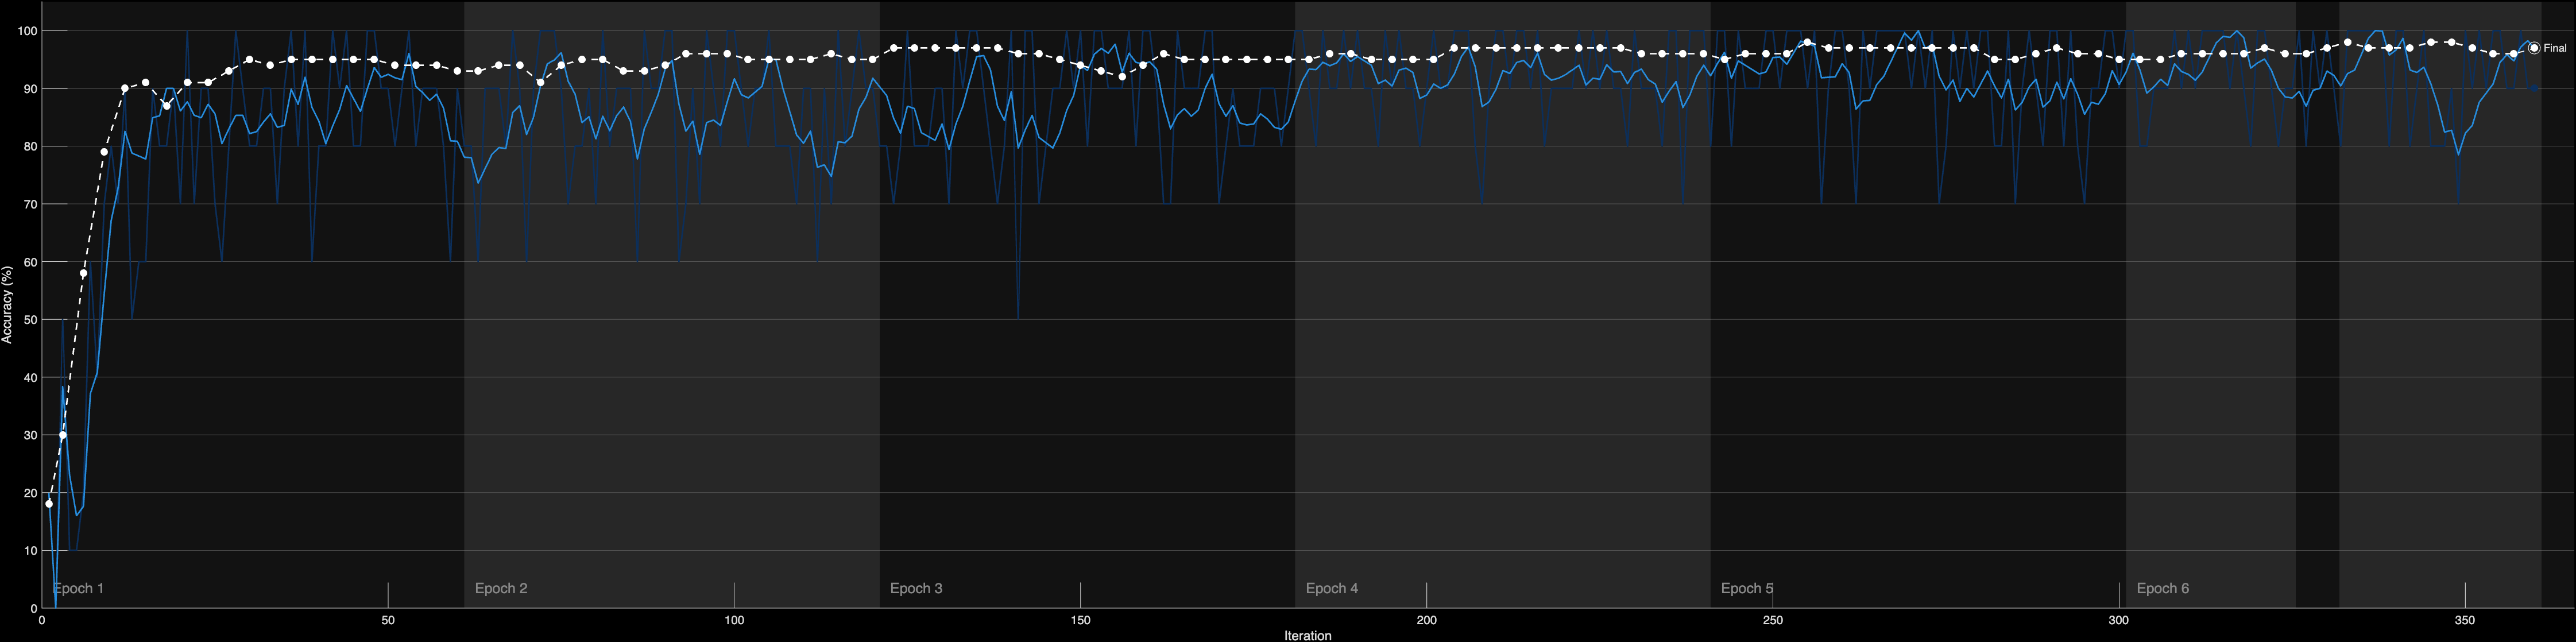
\includegraphics[width=\columnwidth]{images/training}
        \caption{Grafico del training}
    \end{figure}
    \begin{figure}[H]
        \centering
        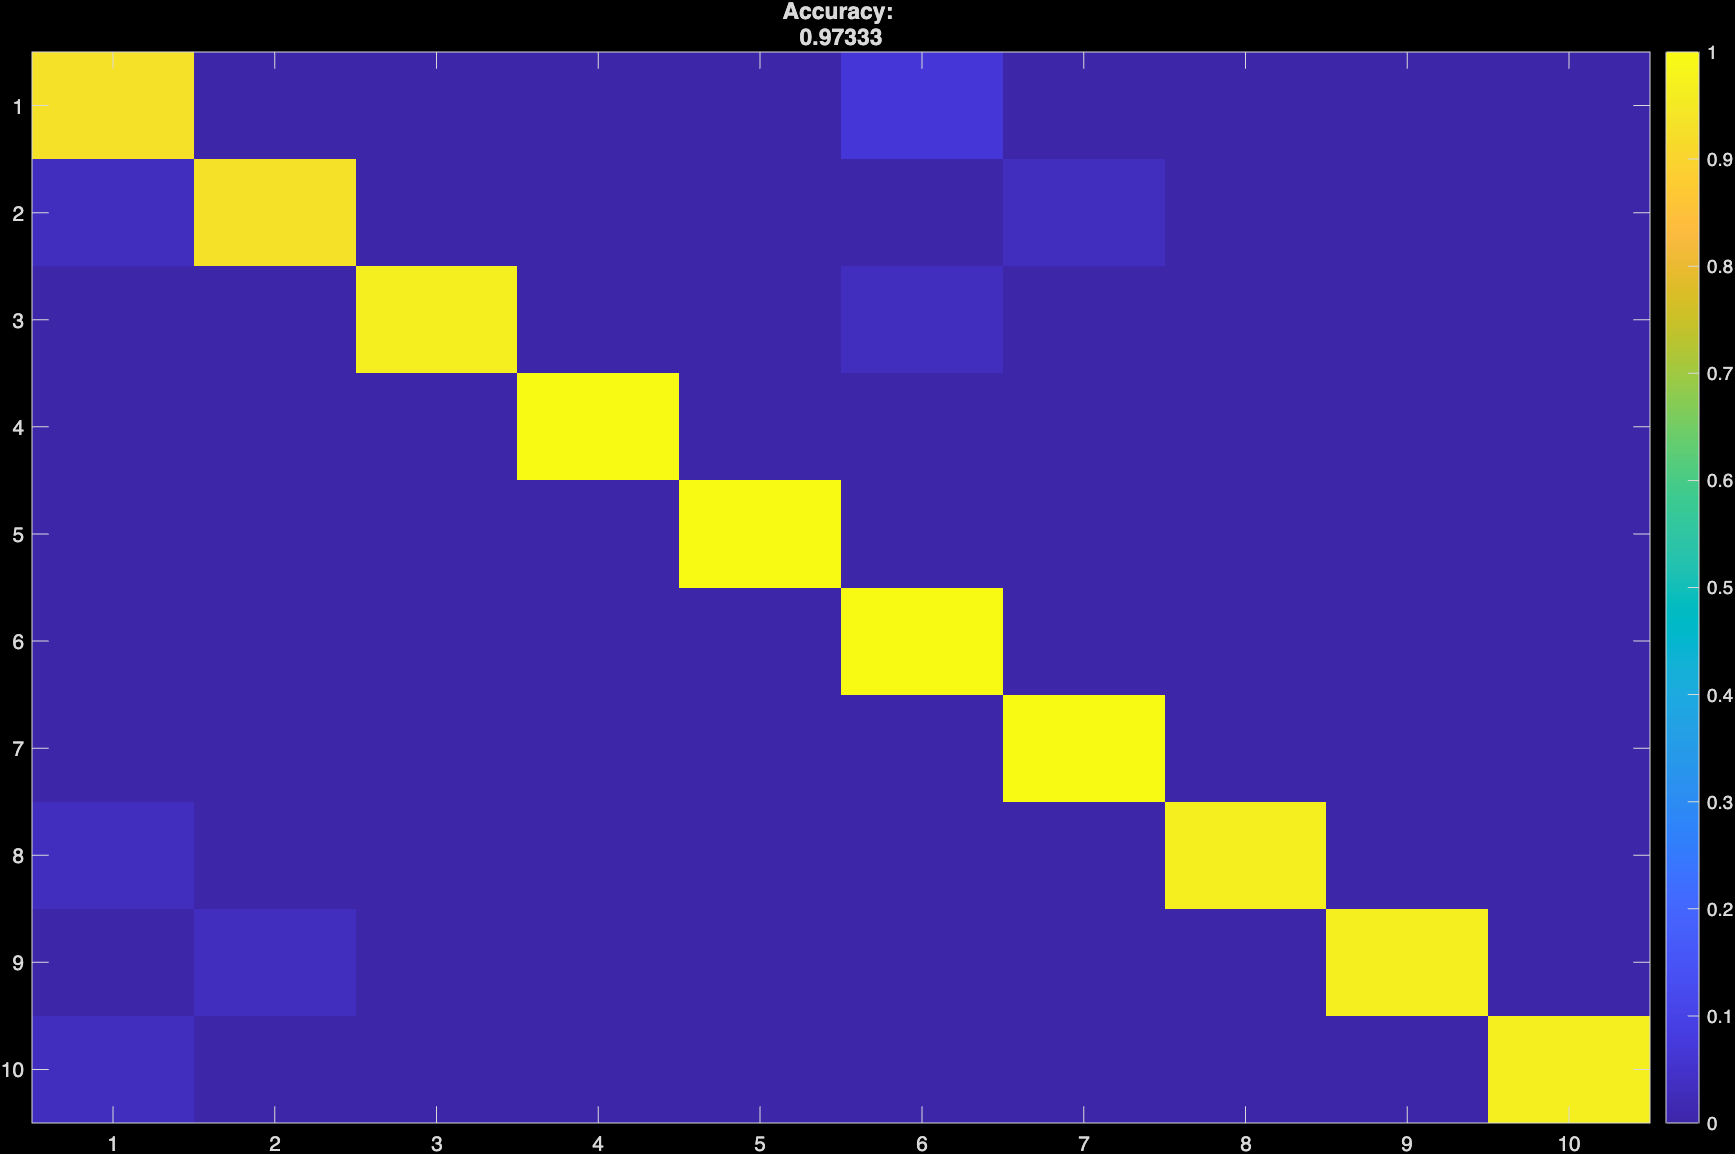
\includegraphics[width=\columnwidth]{images/confusionMatrix}
        \caption{Matrice di confusione}
    \end{figure}
    \newpage
	\section{Codice}
    \lstinputlisting[language=Matlab]{../TL_ft_assignment.m}
\end{document}
